% \[
% \begin{aligned}
%     \hat{u}_x &= \frac{M}{EI} xy \\
%     \hat{u}_y &= \frac{-M}{EI}(\nu x^2 + y^2 - z^2) \\
%     \hat{u}_z &= \frac{-M}{EI} yz
% \end{aligned}
% \]
\begin{figure}[H]
    \centering
    \begin{subfigure}[c]{0.6\linewidth}
        \ExampleFigure{frame-1020}
    \end{subfigure}
    \begin{subfigure}[c]{0.3\linewidth}
        \SectionFigure[width=\linewidth]{HalfFlange}
    \end{subfigure}
    \caption{Model  for Example~\ref{sec:frame-0001}.}
    \label{fig:frame-0001}
\end{figure}

\begin{figure}
\hypertarget{fig:area-graph}{%
\centering
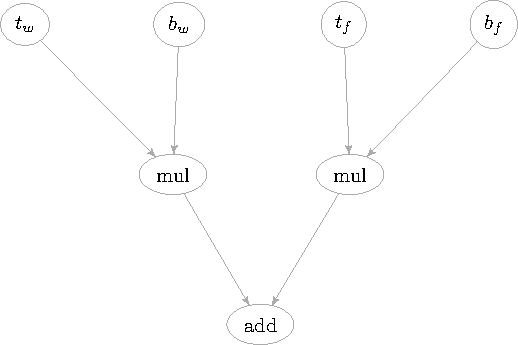
\includegraphics{Examples/frame-0001/img/area.pdf}
\caption{Computational graph for the area of a T-section.}\label{fig:area-graph}
}
\end{figure}
